%
% bewegung.tex -- Begründet die Bewegung von Wirbelringen
%
% !TEX root = ../../buch.tex
% !TEX encoding = UTF-8
%
\section{Bewegung eines Wirbelrings\label{Wirbelringe:Bewegung}}

Bisher wurde die Bewegung eines Wirbelrings noch nicht weiter betrachtet. 
Doch wie man bereits bei Rauchringen beobachten kann, bleiben diese nicht an einem Ort stehen, sondern bewegen sich. 
Um diese Verhalten zu begründen, kann das Biot-Savart-Gesetz \cite{Wirbelringe:FuehrerdurchdieStroemungslehre} angewendet werden, was im folgenden Abschnitt gemacht werden soll.

\subsection{Biot-Savart-Gesetz}

Das Biot-Savart-Gesetz
\[
d \vec{B}
=
\frac{\mu_0}{4\pi}\frac{I \,d \vec{l} \times \vec{r}}{\left\lvert \vec{r}^{\,3}\right\rvert }
\]  % Note : diese Definition weicht von der Definiton 3.2 im ELT2 Skript ab da dort ein Richtungsvektor verwendet wird -> ein r (dort ein R) kürzt sich heraus
wird typischerweise in der Elektrotechnik angewendet, um das Magnetfeld von bewegten Ladungen zu beschreiben (hier nur auf einen Strom durch einen Leiter vereinfacht).
Es kann nur bei geschlossenen Stromkreisen verwendet werden. 

Damit wir das Gesetz nutzen können, müssen wir zunächst die Grössen anpassen und überprüfen, ob das überhaupt erlaubt ist. 
Die elektrodynamischen Grössen haben jeweils ein Gegenstück in der Strömungsmechanik:

\begin{center}
    \begin{tabular}{lcl}
    stromdurchflossener Leiter          & \(\Leftrightarrow \) & Wirbelfaden \\
    Stromstärke \(I\)                   & \(\Leftrightarrow \) & Zirkulation \(\Gamma\) \\
    Stromdichtevektor \(\hat{j}\)       & \(\Leftrightarrow \) & Wirbelstärkevektor \(\vec{\omega}\)\\
    magnetische Feldstärke \(\vec{H}\)  & \(\Leftrightarrow \) & Geschwindigkeit \(\vec{u}\) \\
    \end{tabular}
\end{center}

Im Folgenden wird der Wirbelstärkevektor nicht verwenden.
Jedoch ist der Zusammenhang vom Wirbelstärkevektor zum Stromdichtevektor etwas intuitiver als die Zirkulation zur Stromstärke.

Die Maxwellgleichungen (siehe Abschnitt \ref{chapter:maxwell}) sehen vor das \(\vec{B}\) Feld quellenfrei ist. 
Da wir nur inkompressible Fluide betrachten, ist dies gegeben.

Setzt man nun die entsprechenden Grössen in das Biot-Savart-Gesetz
\[
d\, \vec{u}
=
\frac{\Gamma}{4\pi}\frac{d\, \vec{l} \times \vec{r}}{\left\lvert \vec{r}^{\,3}\right\rvert }
\]
ein, lässt sich damit die Geschwindigkeitsänderung eines Punktes durch ein Wirbelfadenelement beschreiben.
Um die Rechnung zu vereinfachen, können wir annehmen, dass der Wirbelfaden vergleichsweise dünn ist, verglichen zum Durchmesser des Rings aus der Wirbellinie.
Mit dem Integral über diesen Wirbelfaden
\[
\vec{u}
=
\int_{\text{Wirbellinie}} \frac{\Gamma}{4\pi}\frac{d\, \vec{l} \times \vec{r}}{\left\lvert \vec{r}^{\,3}\right\rvert}
\]
erhalten wir die induzierte Geschwindigkeit, welche durch den Wirbelfaden entsteht.
Da dieses Gesetz aus der Elektrotechnik stammt, spricht man in der Strömungsmechanik von einer induzierten Geschwindigkeit.

Um nun die selbstinduzierte Geschwindigkeit zu berechnen, wählen wir ein in der X-Y Plane liegender Wirbelring mit Radius \(a\).
Der Radius des Wirbelfaden ist einfachheitshalber verglichen zum Radius der Wirbellinie vernachlässigbar klein.
Uns interessiert irgendein Punkt, der auf der Wirbellinie liegt.
Somit ist
\(
\vec{r} = 
\begin{pmatrix}
    a\\
    0\\
    0    
\end{pmatrix}\)
und
\(
d\,\vec{l} = 
\begin{pmatrix}
    0\\
    a\\
    0    
\end{pmatrix}d\,\varphi \). 
Setzt man diese in
\[
\vec{u}
=
\int_{0}^{2\pi} \frac{\Gamma }{4\pi}\frac{d\, \vec{l} \times \vec{r}}{\left\lvert \vec{r}^{\,3}\right\rvert },
\]
ein erhält man 
\[
\vec{u}
=
\frac{\Gamma a^{2}}{4\pi a^{3}} \int_{0}^{2\pi} \hat{z}\, d\,\varphi.
\]
Da der Kreisumfang und der Radius immer senkrecht zueinander ist der Richtungsvektor \(\hat{z}\). 
Schlussendlich ergibt sich
\[
\vec{u}
=
\frac{\Gamma }{2 a}\hat{z},
\]
woraus ersichtlich ist das, je kleiner der Wirbelring, desto schneller bewegt er sich.

Würde man dieselbe Rechnung für einen geraden Wirbelfaden durchführen, würde auffallen, dass das Ergebnis für Punkte auf der Wirbellinie null ist.
Der Wirbelfaden induziert sich selbst keine Geschwindigkeit.
Daher, damit sich ein Wirbelfaden von sich bewegt, muss dieser zumindest ein wenig gekrümmt sein.
Ein zweiter Wirbelfaden würde zu einer induzierten Geschwindigkeit führen. 
Dies betrachten wir hier aber nicht weiter. 

\subsection{Bewegung eines Teilchens}

\begin{figure}
\centering
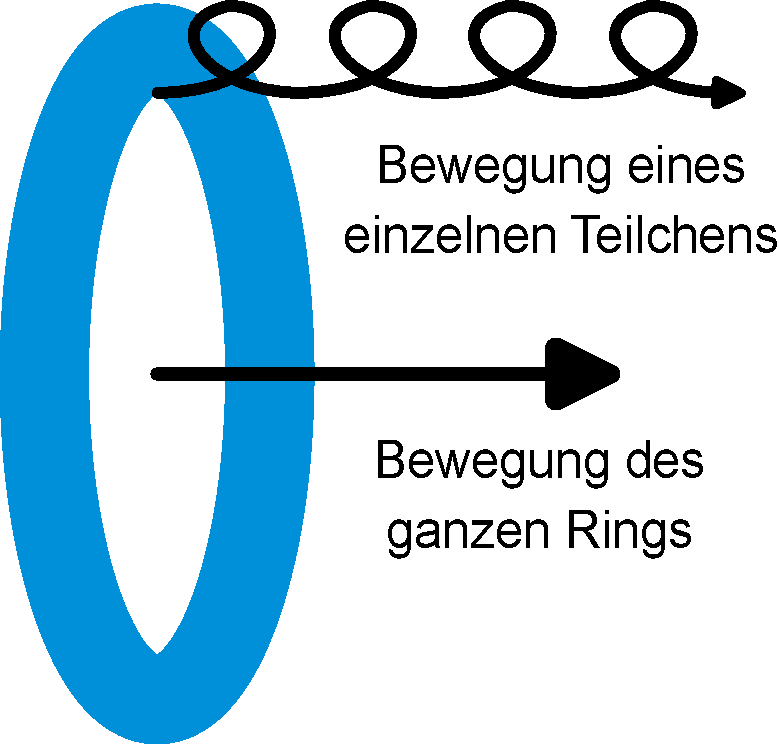
\includegraphics[width=0.4\textwidth]{papers/wirbelringe/fig/ausbreitung_teilchen.pdf}
\caption{Bewegung eines einzelnen Teilchen ToDo besseri Farb für de Ring??? \label{buch:papers:Wirbelringe:fig:ausbreitung_teilchen}}
\end{figure}

Eine interessante Kurve zeichnet sich ab, wenn man ein einzelnes Teilchen beobachtet.
Es bildet sich eine Zykloide.
Die Grösse der Zykloide hängt von der Höhe der Zirkulation ab.
Dies ist in Abbildung \ref{Wirbelringe:fig:ausbreitung_teilchen} dargestellt.
